\documentclass[margin=1mm]{standalone}

%\usepackage{amsmath,amssymb,latexsym,float,epsfig,hyperref}
%\usepackage{framed,color,url,fancybox,fullpage,booktabs,subfigure,wrapfig,chngpage,setspace}

\usepackage[latin1]{inputenc}
\usepackage{tikz}

\usetikzlibrary{shapes,arrows}
\usetikzlibrary{arrows,positioning,mindmap} 
\usetikzlibrary{calc,trees,positioning,arrows,chains,shapes.geometric,%
decorations.pathreplacing,decorations.pathmorphing,shapes,%
matrix,shapes.symbols,plotmarks,decorations.markings,shadows}
\usetikzlibrary{patterns}

\tikzstyle{decision} = [diamond, draw, fill=gray!10,
  text width=6em, text badly centered, node distance=2.5cm, 
  inner sep=0pt,minimum height=1em,text centered]
\tikzstyle{block} = [rectangle, draw, fill=blue!20,
  text width=10em, text centered, rounded corners, minimum height=3.0em]

\tikzstyle{autoblock} = [rectangle, draw, fill=blue!20, text centered, rounded corners]

\tikzstyle{cloud} = [draw, ellipse,fill={rgb:orange,1;yellow,1;pink,1}, node distance=4cm,
    minimum height=1em,text centered]
\tikzstyle{circ} = [draw,circle,fill={rgb:orange,1;yellow,1;pink,1}, 
  node distance=4cm, minimum height=2em, text centered]

\tikzstyle{line} = [draw, very thick, color=black!50, -latex']
\tikzstyle{redline} = [draw, very thick, color=black!50, -latex']
\tikzstyle{dotline} = [draw,dotted, very thick, color=black!50, -latex']

\tikzset{
    poly/.style={
        draw, 
        shape border rotate=0,
        regular polygon,
        regular polygon sides=3,
        fill=red,
        node distance=2cm,
        minimum height=4em, 
    }
}

\tikzstyle{line} = [draw, very thick, color=black, -latex']
\tikzstyle{redline} = [draw, very thick, color=red, -latex']
\tikzstyle{dotline} = [draw,dotted, very thick, color=black!50, -latex']


% find center of two nodes
% https://tex.stackexchange.com/questions/71478/how-to-center-one-node-exactly-between-two-others-with-tikz
\tikzset{
    between/.style args={#1 and #2}{
         at = ($(#1)!0.5!(#2)$)
    }
}

%\tikzset{
%between base/.style args={#1 and #2}{
%between=#1.base and #2.base
%}
%}


% https://tex.stackexchange.com/questions/72784/arrow-with-two-colors-with-tikz
\tikzset{
  double arrow/.style args={#1 colored by #2 and #3}{
    -stealth,line width=#1,#2, % first arrow
    postaction={draw,-stealth,#3,line width=(#1)/3,
                shorten <=(#1)/3,shorten >=2*(#1)/3}, % second arrow
  }
}

\tikzset{
  double -latex/.style args={#1 colored by #2 and #3}{    
    -latex,line width=#1,#2,
    postaction={draw,-latex,#3,line width=(#1)/3,shorten <=(#1)/4,shorten >=4.5*(#1)/3},
  },
  double round cap-latex/.style args={#1 colored by #2 and #3}{    
    round cap-latex,line width=#1,#2,
    postaction={draw,round cap-latex,#3,line width=(#1)/3,shorten <=(#1)/4,shorten >=4.5*(#1)/3},
  },
  double round cap-stealth/.style args={#1 colored by #2 and #3}{
    round cap-stealth,line width=#1,#2,
    postaction={round cap-stealth,draw,,#3,line width=(#1)/3,shorten <=(#1)/3,shorten >=2*(#1)/3},
  },
  double -stealth/.style args={#1 colored by #2 and #3}{
    -stealth,line width=#1,#2,
    postaction={-stealth,draw,,#3,line width=(#1)/3,shorten <=(#1)/3,shorten >=2*(#1)/3},
  },
}


\makeatletter 
\@namedef{color@1}{red!40}
\@namedef{color@2}{green!40}   
\@namedef{color@3}{blue!40} 
\@namedef{color@4}{cyan!40}  
\@namedef{color@5}{magenta!40} 
\@namedef{color@6}{yellow!40}    

\newcommand{\graphitemize}[2]{%
  \begin{tikzpicture}[at start, every node/.style={align=center}]  
    \node[minimum size=5cm,circle,
%    fill=gray!40,
ultra thick,
 fill = white,
 text  = black,
 draw = black,
    font=\Large, outer sep=1cm,inner sep=.5cm](ce){#1};  
    \foreach \gritem [count=\xi] in {#2}
             {\global\let\maxgritem\xi}  
             \foreach \gritem [count=\xi] in {#2}
                      {% 
                        \pgfmathtruncatemacro{\angle}{360/\maxgritem*\xi}
                        \edef\col{\@nameuse{color@\xi}}
                        \node[circle,
                        font=\bfseries\Large,    
                          ultra thick,
                          draw=white,
                          %                          fill opacity=.75,
                          fill = black,
                          text = white,
                          minimum size=3cm] at (ce.\angle) {\gritem };}%
  \end{tikzpicture}  
}%

\tikzset{
  ring shading/.code args={from #1 at #2 to #3 at #4}{
    \def\colin{#1}
    \def\radin{#2}
    \def\colout{#3}
    \def\radout{#4}
    \pgfmathsetmacro{\proportion}{\radin/\radout}
    \pgfmathsetmacro{\outer}{.8818cm}
    \pgfmathsetmacro{\inner}{.8818cm*\proportion}
    \pgfmathsetmacro{\innerlow}{\inner-0.01pt}
    \pgfdeclareradialshading{ring}{\pgfpoint{0cm}{0cm}}%
    {
      color(0pt)=(white);
      color(\innerlow)=(white);
      color(\inner)=(#1);
      color(\outer)=(#3)
    }
    \pgfkeysalso{/tikz/shading=ring}
  },
}


\usepackage[standard-baselineskips]{cmbright}
\renewcommand\familydefault{\sfdefault}
\usepackage[T1]{fontenc}

% % % \include{tableau_colors} in your .tex file to use these custom
% Tableau colors
% https://gist.github.com/AndiH/c957b4d769e628f506bd

\definecolor{dblue}{RGB}{31, 119, 180}
\definecolor{lblue}{RGB}{174, 199, 232}

\definecolor{dorange}{RGB}{255, 127, 14}
\definecolor{lorange}{RGB}{255, 187, 120}

\definecolor{dgreen}{RGB}{44, 160, 44}
\definecolor{lgreen}{RGB}{152, 223, 138}

\definecolor{dred}{RGB}{214, 39, 40}
\definecolor{lred}{RGB}{255, 152, 150}

\definecolor{dpurple}{RGB}{148, 103, 189} 
\definecolor{lpurple}{RGB}{197, 176, 213}

\definecolor{dbrown}{RGB}{140, 86, 75} 
\definecolor{lbrown}{RGB}{196, 156, 148}    

\definecolor{dpink}{RGB}{227, 119, 194}
\definecolor{lpink}{RGB}{247, 182, 210}

\definecolor{dgray}{RGB}{127, 127, 127}
\definecolor{lgray}{RGB}{199, 199, 199}

\definecolor{dolive}{RGB}{188, 189, 34}
\definecolor{lolive}{RGB}{219, 219, 141}

\definecolor{dskyblue}{RGB}{23, 190, 207}
\definecolor{lskyblue}{RGB}{158, 218, 229}

\definecolor{gold}{RGB}{255,223,0}
 in your .tex file to use these custom
% Tableau colors
% https://gist.github.com/AndiH/c957b4d769e628f506bd

\definecolor{dblue}{RGB}{31, 119, 180}
\definecolor{lblue}{RGB}{174, 199, 232}

\definecolor{dorange}{RGB}{255, 127, 14}
\definecolor{lorange}{RGB}{255, 187, 120}

\definecolor{dgreen}{RGB}{44, 160, 44}
\definecolor{lgreen}{RGB}{152, 223, 138}

\definecolor{dred}{RGB}{214, 39, 40}
\definecolor{lred}{RGB}{255, 152, 150}

\definecolor{dpurple}{RGB}{148, 103, 189} 
\definecolor{lpurple}{RGB}{197, 176, 213}

\definecolor{dbrown}{RGB}{140, 86, 75} 
\definecolor{lbrown}{RGB}{196, 156, 148}    

\definecolor{dpink}{RGB}{227, 119, 194}
\definecolor{lpink}{RGB}{247, 182, 210}

\definecolor{dgray}{RGB}{127, 127, 127}
\definecolor{lgray}{RGB}{199, 199, 199}

\definecolor{dolive}{RGB}{188, 189, 34}
\definecolor{lolive}{RGB}{219, 219, 141}

\definecolor{dskyblue}{RGB}{23, 190, 207}
\definecolor{lskyblue}{RGB}{158, 218, 229}

\definecolor{gold}{RGB}{255,223,0}
 in your .tex file to use these custom
% Tableau colors
% https://gist.github.com/AndiH/c957b4d769e628f506bd

\definecolor{dblue}{RGB}{31, 119, 180}
\definecolor{lblue}{RGB}{174, 199, 232}

\definecolor{dorange}{RGB}{255, 127, 14}
\definecolor{lorange}{RGB}{255, 187, 120}

\definecolor{dgreen}{RGB}{44, 160, 44}
\definecolor{lgreen}{RGB}{152, 223, 138}

\definecolor{dred}{RGB}{214, 39, 40}
\definecolor{lred}{RGB}{255, 152, 150}

\definecolor{dpurple}{RGB}{148, 103, 189} 
\definecolor{lpurple}{RGB}{197, 176, 213}

\definecolor{dbrown}{RGB}{140, 86, 75} 
\definecolor{lbrown}{RGB}{196, 156, 148}    

\definecolor{dpink}{RGB}{227, 119, 194}
\definecolor{lpink}{RGB}{247, 182, 210}

\definecolor{dgray}{RGB}{127, 127, 127}
\definecolor{lgray}{RGB}{199, 199, 199}

\definecolor{dolive}{RGB}{188, 189, 34}
\definecolor{lolive}{RGB}{219, 219, 141}

\definecolor{dskyblue}{RGB}{23, 190, 207}
\definecolor{lskyblue}{RGB}{158, 218, 229}

\definecolor{gold}{RGB}{255,223,0}


\usepackage{smartdiagram}

\begin{document}

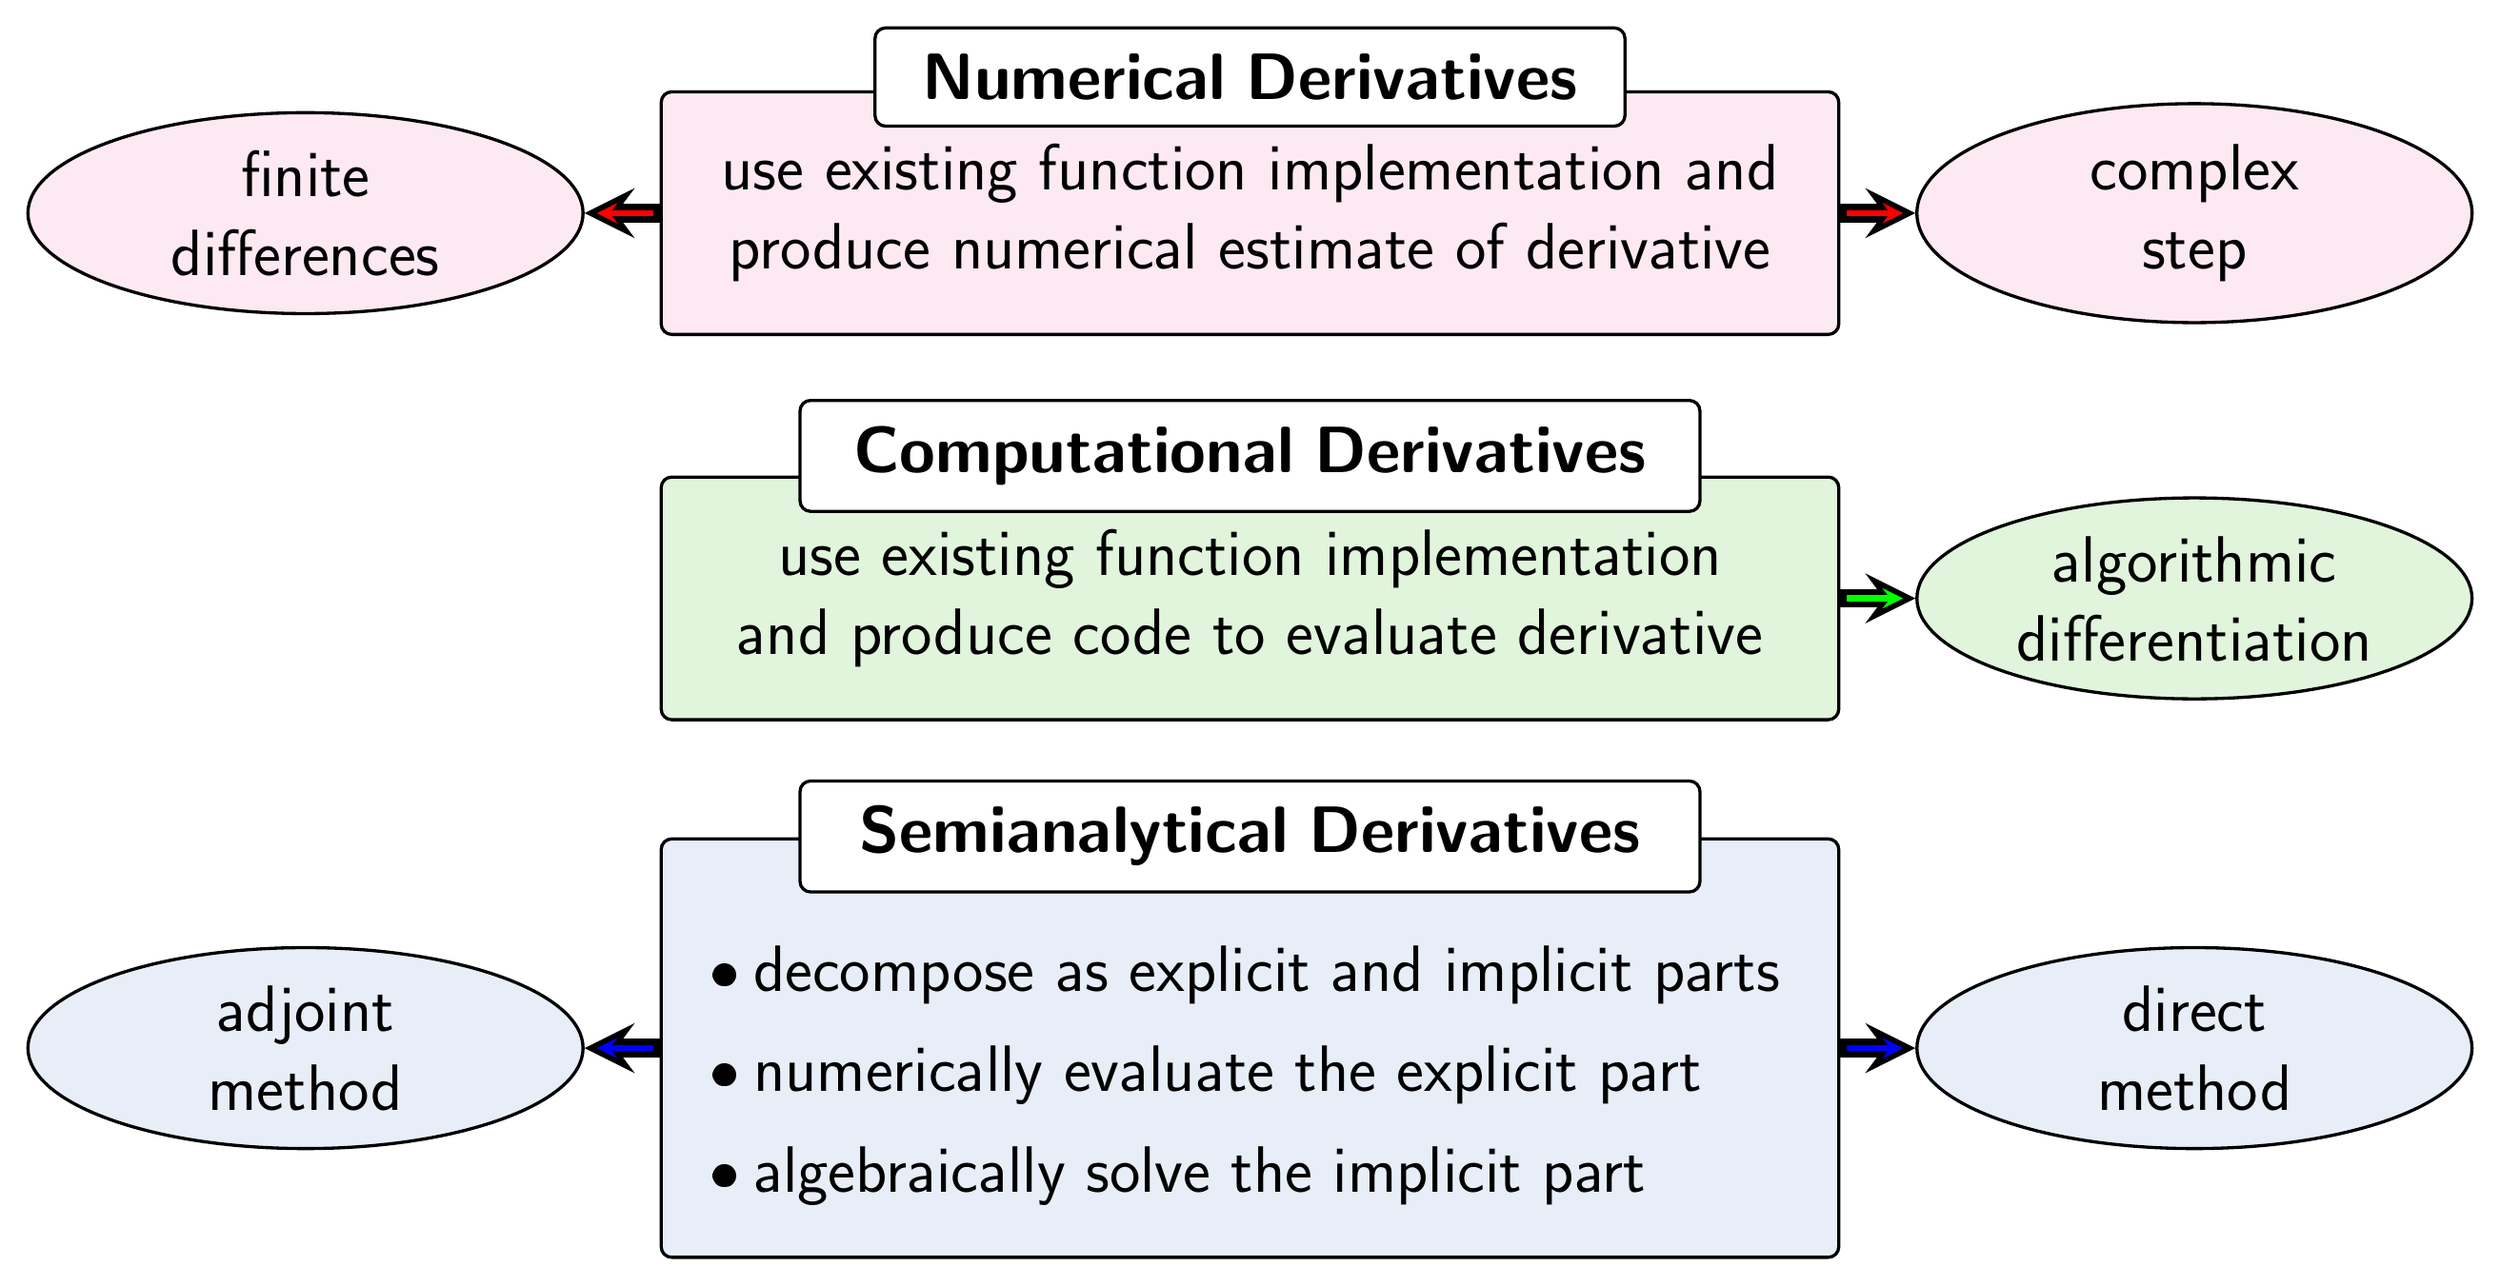
\begin{tikzpicture}[auto]

  %%%%%%%%%%%%%%%%%%%%%%%%%%%%%%%%%%%%%%%%%%%%%%%%%%%%%%%%%%%%%%
  %                   NUMERICAL DERIVATIVES                    %
  %%%%%%%%%%%%%%%%%%%%%%%%%%%%%%%%%%%%%%%%%%%%%%%%%%%%%%%%%%%%%%
  
  \node [block, very thick, 
    node distance=4.0cm, 
    inner ysep=2em, 
    inner xsep=1em, 
    text width=15cm,
    fill=lpink!30,
    font=\Huge] at (0,0) (numerical-principle) {
    use existing function implementation and produce numerical estimate of derivative
  };
  \node [block, very thick, 
    node distance=0.0cm, 
    inner ysep=1em,
    inner xsep=0em, 
    text width=10cm,
    fill=white,
    font=\Huge, above = -0.5cm of numerical-principle] (numerical-header) {
    \textbf{Numerical Derivatives}
  };
  \node [cloud , very thick, node distance=5cm, text width=5cm, fill=lpink!30, font=\Huge, left = 1cm of numerical-principle] (fdm) {finite differences}; 
  \draw[double arrow=7pt colored by black and red] (numerical-principle) -- (fdm);  
  \node [cloud , very thick, node distance=5cm, text width=5cm, fill=lpink!30, font=\Huge, right = 1cm of numerical-principle] (csm) {complex \\ step}; 
  \draw[double arrow=7pt colored by black and red] (numerical-principle) -- (csm);

  %%%%%%%%%%%%%%%%%%%%%%%%%%%%%%%%%%%%%%%%%%%%%%%%%%%%%%%%%%%%%%
  %                   COMPUTATIONAL  DERIVATIVES               %
  %%%%%%%%%%%%%%%%%%%%%%%%%%%%%%%%%%%%%%%%%%%%%%%%%%%%%%%%%%%%%%
  
  \node [block, very thick, 
    node distance=4.0cm, 
    inner ysep=2em, 
    inner xsep=1em, 
    text width=15cm,
    fill=lgreen!30,
    font=\Huge, below = 3.5cm] (computational-principle) {
    use existing function implementation and produce code to evaluate derivative    
  };
  \node [block, very thick, 
    node distance=0.0cm, 
    inner ysep=1em,
    inner xsep=0em, 
    text width=12cm,
    fill=white!25,
    font=\Huge, above = -0.5cm of computational-principle] (computational-header) {
    \textbf{Computational Derivatives}
  };
  \node [cloud , very thick, node distance=5cm, text width=5cm, fill=lgreen!30, font=\Huge, right = 1cm of computational-principle] (adm) {algorithmic \\differentiation}; 
  \draw[double arrow=7pt colored by black and green] (computational-principle) -- (adm);  

  %%%%%%%%%%%%%%%%%%%%%%%%%%%%%%%%%%%%%%%%%%%%%%%%%%%%%%%%%%%%%%
  %                   SEMIANALYTIC DERIVATIVES                 %
  %%%%%%%%%%%%%%%%%%%%%%%%%%%%%%%%%%%%%%%%%%%%%%%%%%%%%%%%%%%%%%
  
  \node [block, very thick, 
    node distance=6.0cm, 
    inner ysep=2em, 
    inner xsep=1em, 
    text width=15cm,
    fill=lblue!30,
    font=\Huge, below of = computational-principle] (analytical-principle) {
    \begin{itemize}
      \item decompose as explicit and implicit parts
      \item numerically evaluate the explicit part
      \item algebraically solve the implicit part
      %\item evaluate function and corresponding derivative when subject to implicit constraint on state variables
    \end{itemize}
  };
  \node [block, very thick, 
    node distance=0.0cm, 
    inner ysep=1em,
    inner xsep=0em, 
    text width=12cm,
    fill=white!25,
    font=\Huge, above = -0.75cm of analytical-principle] (analytical-header) {
    \textbf{Semianalytical Derivatives}
  };
  \node [cloud , very thick, node distance=5cm, text width=5cm, fill=lblue!30, font=\Huge, left = 1cm of analytical-principle] (adjoint) {adjoint \\ method}; 
  \draw[double arrow=7pt colored by black and blue] (analytical-principle) -- (adjoint);  
  \node [cloud , very thick, node distance=5cm, text width=5cm, fill=lblue!30, font=\Huge, right = 1cm of analytical-principle] (direct) {direct \\ method}; 
  \draw[double arrow=7pt colored by black and blue] (analytical-principle) -- (direct);

\end{tikzpicture}

\end{document}
